


% Define custom colors for code blocks
\definecolor{codegray}{gray}{0.9}
\definecolor{codegreen}{rgb}{0,0.6,0}
\definecolor{codeblue}{rgb}{0,0,0.6}
\definecolor{codepurple}{rgb}{0.58,0,0.82}

% Define custom style for directory listing
\lstdefinelanguage{Tree}{
  moredelim=**[is][\color{blue}]{|}{|}
}

\lstdefinestyle{tree}{
  language=Tree,
  basicstyle=\ttfamily\small,
  showspaces=false,
  showstringspaces=false,
  breaklines=true,
  frame=single,
  backgroundcolor=\color{gray!10},
}


% Define TypeScript as a language
\lstdefinelanguage{typescript}{
  keywords={interface, string, number, boolean, Date, undefined, null, any, void, never, readonly, public, private, protected},
  keywordstyle=\color{codeblue}\bfseries,
  ndkeywords={_id, name, description, location, createdAt, imageUrl, startDateTime, endDateTime, price, isFree, url, category, organizer, stripeId, totalAmount, event, buyer, firstName, lastName, photo, username, clerkId, email},
  ndkeywordstyle=\color{codepurple}\bfseries,
  identifierstyle=\color{black},
  sensitive=true,
  comment=[l]{//},
  morecomment=[s]{/*}{*/},
  commentstyle=\color{codegreen}\ttfamily,
  stringstyle=\color{codepurple}\ttfamily,
  morestring=[b]',
  morestring=[b]"
}

% Set the default style for TypeScript code
\lstdefinestyle{typescript}{
  language=typescript,
  backgroundcolor=\color{codegray},
  basicstyle=\ttfamily\small,
  breaklines=true,
  frame=single,
  numbers=left,
  numberstyle=\tiny\color{gray},
  numbersep=5pt
}
\chapter{Developer documentation}
\label{ch:impl}

This project is designed as a modern \textbf{Next.js full-stack application}, utilizing a monolithic architecture pattern. Instead of separating the front-end and back-end into different repositories, the application consolidates all components into a single repository. 

This architectural choice provides several advantages:

\begin{itemize}
    \item All code resides in a single repository, simplifying development workflows.
    \item Seamless type sharing between client and server components.
    \item Easier deployment and maintenance as a single cohesive unit.
\end{itemize}

\section{Components of design}

\subsection{Use Case Diagram}
The use case diagram represents the interactions between various users of the event management system—\textbf{System Admin}, \textbf{Event Organizer}, and \textbf{Event Attendee}—and the functionalities available to them. Key use cases and relationships include:  

\begin{itemize}
    \item \textbf{Category Management:}  
    The \textbf{System Admin} can manage event categories, such as adding, updating, or removing categories.  

    \item \textbf{Event Management:}  
    \begin{itemize}
        \item The \textbf{Event Organizer} has the ability to create, update, delete, and view events.  
        \item While creating an event, organizers can optionally extend the functionality to include uploading event images or creating new categories.  
        \item Event organizers can also filter and search for events by category.  
    \end{itemize}

    \item \textbf{Order Management:}  
    \begin{itemize}
        \item The \textbf{Event Attendee} can purchase tickets for events and view their orders.  
        \item The purchase ticket flow includes processing payments via an external payment system (e.g., Stripe).  
    \end{itemize}

    \item \textbf{Authentication:}  
    Both \textbf{Event Organizer} and \textbf{Event Attendee} can sign up, sign in, and manage their profiles.  
\end{itemize}

\textbf{Relationships:}  
\begin{itemize}
    \item \textit{Extends:} Optional flows like uploading event images or creating categories are represented as extensions to the main event management flow.  
    \item \textit{Includes:} Common actions like processing payments or uploading files are modularized into reusable flows.  
\end{itemize}

\begin{figure}[H]
	\centering	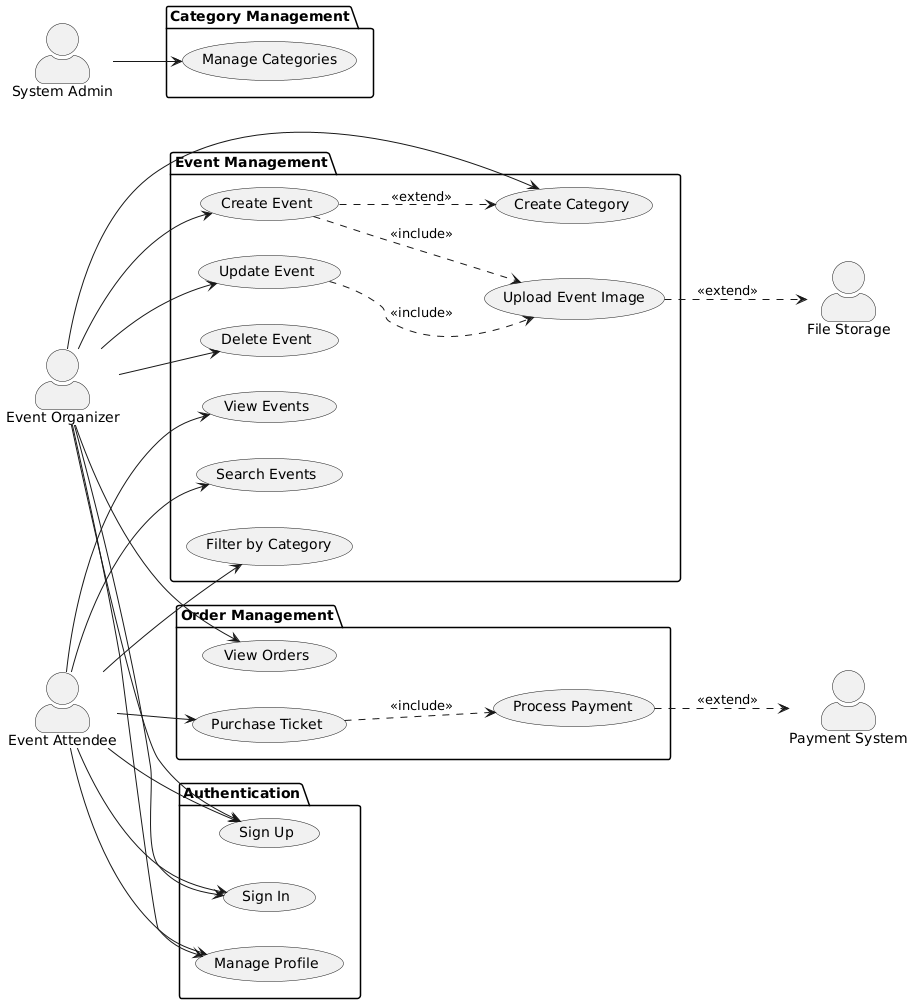
\includegraphics[width=1.0\textwidth,height=500px,frame]{usecase.png}
    \caption{Use Case Diagram}
    \end{figure}


\subsection{UML Class Diagram}  
The UML class diagram provides a clear representation of the core entities in the event management system and their relationships. These entities include \textbf{User}, \textbf{Order}, \textbf{Event}, and \textbf{Category}. The diagram can be summarized as follows:  

\begin{itemize}
    \item \textbf{User:}  
    \begin{itemize}
        \item Fields: \texttt{\_id}, \texttt{clerkId}, \texttt{email}, \texttt{username}, \texttt{firstName}, \texttt{lastName}, \texttt{photo}.  
        \item Represents users in the system and handles authentication and profile management.  
    \end{itemize}
    
    \item \textbf{Order:}  
    \begin{itemize}
        \item Fields: \texttt{\_id}, \texttt{createdAt}, \texttt{stripeId}, \texttt{totalAmount}.  
        \item Represents event bookings and manages payments for tickets.  
    \end{itemize}
    
    \item \textbf{Event:}  
    \begin{itemize}
        \item Fields: \texttt{\_id}, \texttt{title}, \texttt{description}, \texttt{location}, \texttt{createdAt}, \texttt{imageUrl}, \texttt{startDateTime}, \texttt{endDateTime}, \texttt{price}, \texttt{isFree}, \texttt{url}.  
        \item Core entity representing events, including details about location, time, and cost.  
    \end{itemize}
    
    \item \textbf{Category:}  
    \begin{itemize}
        \item Fields: \texttt{\_id}, \texttt{name}.  
        \item Categorizes events into different types (e.g., workshops, concerts).  
    \end{itemize}
\end{itemize}

\textbf{Relationships:}  
\begin{itemize}
    \item \textbf{User-Order:}  
    A user places multiple orders (one-to-many relationship).  
    \item \textbf{User-Event:}  
    A user can organize multiple events (one-to-many relationship).  
    \item \textbf{Event-Category:}  
    Each event belongs to a single category (many-to-one relationship).  
    \item \textbf{Order-Event:}  
    Orders reference specific events (many-to-one relationship).  
\end{itemize}


\begin{figure}[H]
	\centering	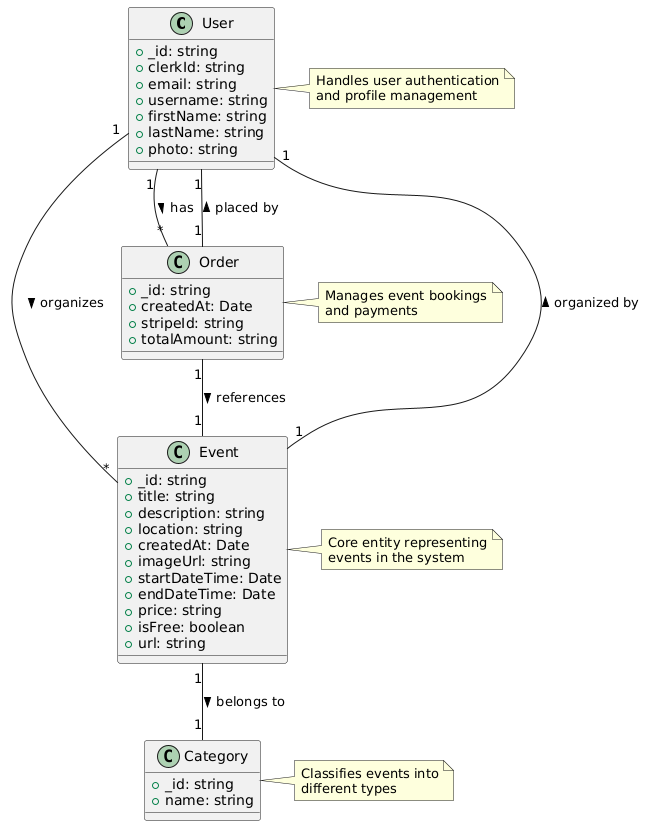
\includegraphics[width=1.0\textwidth,height=500px,frame]{umlclass.png}
    \caption{UML Class Diagram}
    \end{figure}



\subsection{Entity Relationship Diagram (ERD)}

\subsubsection{Overview}
The Event Management Platform's database schema consists of four main entities: \textbf{User}, \textbf{Event}, \textbf{Category}, and \textbf{Order}. The schema is designed to efficiently support event creation, ticket booking, and user management.

\subsubsection{Core Entities}
\paragraph{User}
\begin{itemize}
    \item Stores user profiles and authentication data.
    \item \textbf{Key Fields}: \texttt{id}, \texttt{clerkId}, \texttt{email}, \texttt{username}, \texttt{firstName}, \texttt{lastName}, \texttt{photo}.
    \item Serves as the primary entity for both event organizers and attendees.
\end{itemize}

\paragraph{Event}
\begin{itemize}
    \item Manages event information and scheduling.
    \item \textbf{Key Fields}: \texttt{id}, \texttt{title}, \texttt{description}, \texttt{location}, \texttt{dates}, \texttt{price}, \texttt{imageUrl}.
    \item Links to the event organizer (\texttt{User}) and event category (\texttt{Category}).
\end{itemize}

\paragraph{Category}
\begin{itemize}
    \item Classifies events into various types.
    \item \textbf{Key Fields}: \texttt{id}, \texttt{name}.
    \item Enables event filtering and organization.
\end{itemize}

\paragraph{Order}
\begin{itemize}
    \item Handles ticket purchases and payment processing.
    \item \textbf{Key Fields}: \texttt{id}, \texttt{stripeId}, \texttt{totalAmount}, \texttt{createdAt}.
    \item Links the buyer (\texttt{User}) with the purchased \texttt{Event}.
\end{itemize}

\subsubsection{Key Relationships}
\begin{itemize}
    \item \textbf{User $\rightarrow$ Event (1:N)}: A user can organize multiple events.
    \item \textbf{User $\rightarrow$ Order (1:N)}: A user can make multiple ticket purchases (orders).
    \item \textbf{Event $\rightarrow$ Category (N:1)}: Each event belongs to one category.
    \item \textbf{Event $\rightarrow$ Order (1:N)}: An event can have multiple ticket orders.
\end{itemize}

\subsubsection{Implementation}
\begin{itemize}
    \item The database is built using \textbf{MongoDB} with \textbf{Mongoose ODM}.
    \item Referential integrity is implemented through \texttt{ObjectId} references.
    \item Designed to support efficient querying and data retrieval.
    \item Validation rules and required field constraints are included to ensure data consistency.
\end{itemize}

\begin{figure}[H]
	\centering	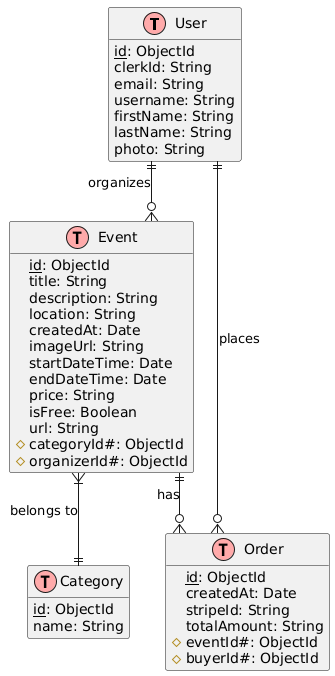
\includegraphics[width=0.6\textwidth,height=450px,frame]{erd.png}
    \caption{Entity Relationship Diagram}
    \end{figure}





\subsection{User Sequence Diagram}

The sequence diagram illustrates the interaction flow between the system components and the user, highlighting key processes such as authentication, event creation, booking, and management. Below is an explanation of each sequence:

\begin{itemize}
    \item \textbf{User Authentication:}
    \begin{itemize}
        \item The user initiates the process by accessing the platform.
        \item The frontend (Next.js) sends a request for authentication to the authentication service (Clerk Auth).
        \item The authentication service returns the session details. For new users, the process involves creating a user record in the database via a webhook triggered by \texttt{user.created}, confirming creation, and updating the user metadata.
    \end{itemize}

    \item \textbf{Event Creation:}
    \begin{itemize}
        \item The user begins the process of creating a new event via the frontend.
        \item An image for the event is uploaded to a file storage service (UploadThing), which returns the image URL.
        \item Event details are then submitted to the backend, where they are stored in the database (MongoDB), and the system confirms the successful storage of data.
        \item The user is shown a success confirmation on the frontend.
    \end{itemize}

    \item \textbf{Event Booking:}
    \begin{itemize}
        \item The user clicks on "Book Event," initiating a checkout session via the backend.
        \item The backend communicates with Stripe to create a session and returns the session URL to the frontend, redirecting the user to the Stripe payment page.
        \item Two possible scenarios:
        \begin{itemize}
            \item \textit{Successful Payment:} Stripe triggers a webhook for payment success. The backend creates an order record in the database, confirms the order and the user is shown a success page.
            \item \textit{Payment Failed:} The user is shown an error message in case of failure.
        \end{itemize}
    \end{itemize}

    \item \textbf{Event Management:}
    \begin{itemize}
        \item The user accesses their dashboard to manage events.
        \item The frontend requests the user's events from the backend.
        \item The backend queries the database for the events and returns the data.
        \item The user is presented with a list of their events.
    \end{itemize}
\end{itemize}


\begin{figure}[H]
	\centering	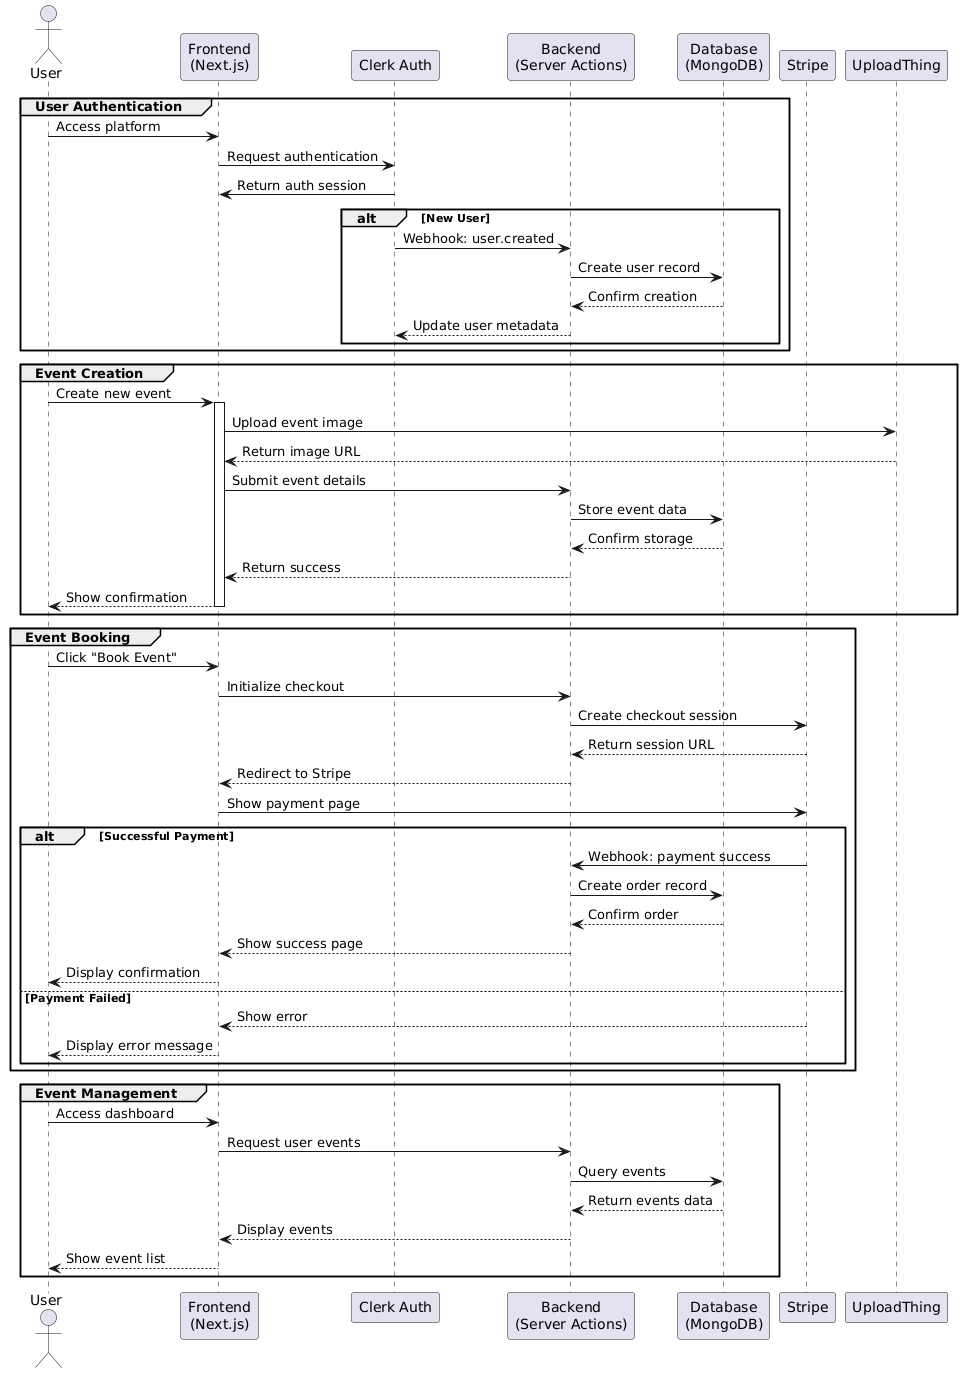
\includegraphics[width=1.0\textwidth,height=700px,frame]{userseq.png}
    \caption{User Sequence Diagram}
    \end{figure}




\section{Implementation}

The technology stack for this project is composed of:

\paragraph{Frontend Technologies}
\begin{itemize}
    \item \textbf{Next.js 14}: Core framework providing both client and server capabilities.
    \item \textbf{TypeScript}: For type-safe code development.
    \item \textbf{Tailwind CSS}: For responsive and utility-first styling.
    \item \textbf{React Hook Form}\cite{reacthookform}: Form management and validation.
    \item \textbf{Zod}\cite{zod}: Schema validation library.
    \item \textbf{RadixUI}\cite{radixui}: Accessible component primitives.
    \item \textbf{React DatePicker}\cite{reactdatepicker}: Date and time selection component.
\end{itemize}

\paragraph{Backend Technologies}
\begin{itemize}
    \item \textbf{MongoDB}: NoSQL database for flexible data storage.
    \item \textbf{Mongoose}: ODM (Object Data Modeling) for MongoDB interaction.
    \item \textbf{Clerk}: Authentication and user management.
    \item \textbf{Stripe}: Payment processing integration.
    \item \textbf{Uploadthing}: File upload and storage solution.
\end{itemize}


\subsection{Hardware Requirements}
Hardware requirements are highly subjective. Most modern computers can handle a medium-sized web project. However, the following specifications are recommended for optimal performance:

\begin{itemize}
    \item \textbf{Processor:} Multi-core CPU
    \item \textbf{RAM:} At least 8 GB
    \item \textbf{Storage:} SSD with at least 256 GB of free space
    \item \textbf{Operating System:} Modern 64-bit OS
\end{itemize}


\subsection{Software Requirements}

The following is the list of software tools used in the development process. After the list, the setup and usage for each of them will be explained.

\begin{itemize}
    \item \textbf{Node.js (v20.12.2):} Used for running the Next.js application.
    \item \textbf{MongoDB:} NoSQL database for flexible and efficient data storage.
    \item \textbf{Stripe:} Payment processing for ticket purchases.
    \item \textbf{Uploadthing:} File upload and storage solution for event images.
    \item \textbf{Clerk:} Authentication and user management.
    \item \textbf{Git:}\cite{git} Version control system for tracking code changes.
\end{itemize}



\subsection{Software Environment Set up}
This section provides detailed instructions on how to install and set up the required software step by step. Please follow these instructions carefully. Once these steps are completed successfully, the development environment will be ready to use.

\begin{enumerate}
    \item \textbf{Node.js Setup:}
    \begin{itemize}
        \item Download the latest stable version of Node.js from \texttt{https://nodejs.org}.
        \item Install it following the on-screen instructions.
        \item Verify installation by running \texttt{node -v} and \texttt{npm -v} in your terminal.
    \end{itemize}
    
    \item \textbf{MongoDB:}
    \newline
    To store data for the application, it is essential to have a MongoDB account and configure the connection URL provided by MongoDB. Follow the steps below to set up MongoDB for your project:
    \begin{enumerate}
    \item \textbf{Create a MongoDB Account:}
    \begin{itemize}
        \item Register an account at \url{https://mongodb.com}.
        \item After logging in, you will be redirected to \url{https://cloud.mongodb.com}.
    \end{itemize}
    
    \item \textbf{Create a Database:}
    \begin{itemize}
        \item Navigate to the \textit{Database} tab.
        \item Click on \textit{Create Database} and follow the prompts as shown in Figure~\ref{fig:create_database}.
    \end{itemize}

    \begin{figure}[H]
	\centering	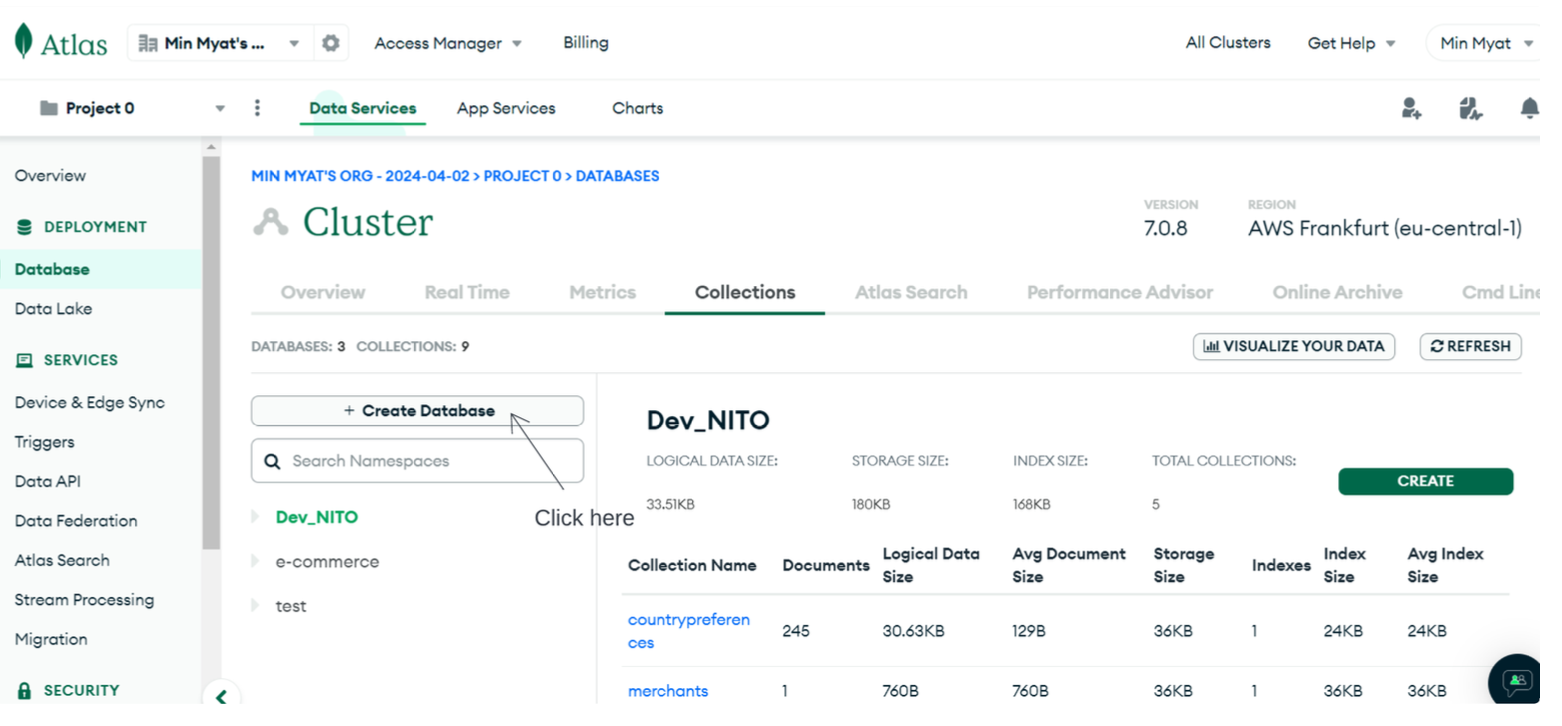
\includegraphics[width=1.0\textwidth,height=300px,frame]{create_database_example.png}
    \caption{How to Create a Database}
    \label{fig:create_database}
    \end{figure}

    \item \textbf{Connect to the Database:}
    \begin{itemize}
        \item Navigate to the \textit{Overview} tab on the left side.
        \item Click on the \textit{Connect} button (see Figure~\ref{fig:connect_database}).
        \item A modal with connection instructions will appear.
    \end{itemize}

    \begin{figure}[H]
	\centering	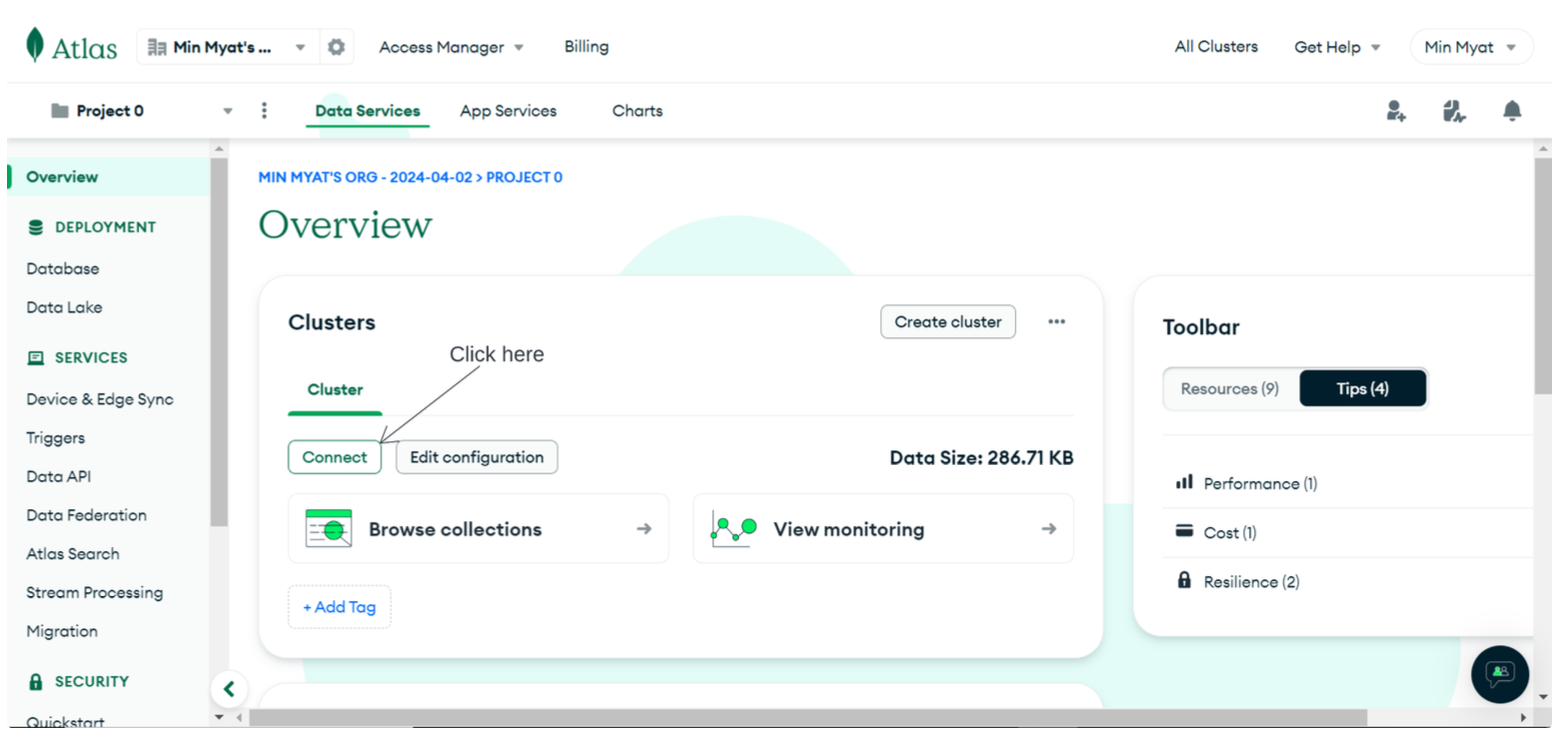
\includegraphics[width=1.0\textwidth,height=300px,frame]
    {connect_database_example.png}
    \caption{How to Connect to the Database}
    \label{fig:connect_database}
    \end{figure}
    
    
    \item \textbf{Modify the Connection String:}
    \begin{itemize}
        \item Copy the connection string provided by MongoDB.
        \item Replace the placeholders in the connection string with your username, password, and database name. Below is an example:
        \lstset{caption={MONGODB connection string}}
\begin{lstlisting}
const url = "mongodb+srv://<username>:<password>
        @cluster0.2cqmiec.mongodb.net/<database-name>?
        retryWrites=true&w=majority&appName=<cluster-name>"
\end{lstlisting}
        \item If the cluster name was customized, it can be found in the \textit{Cluster Name} section (see Figure~\ref{fig:cluster_name}).
    \end{itemize}

    \begin{figure}[H]
	\centering	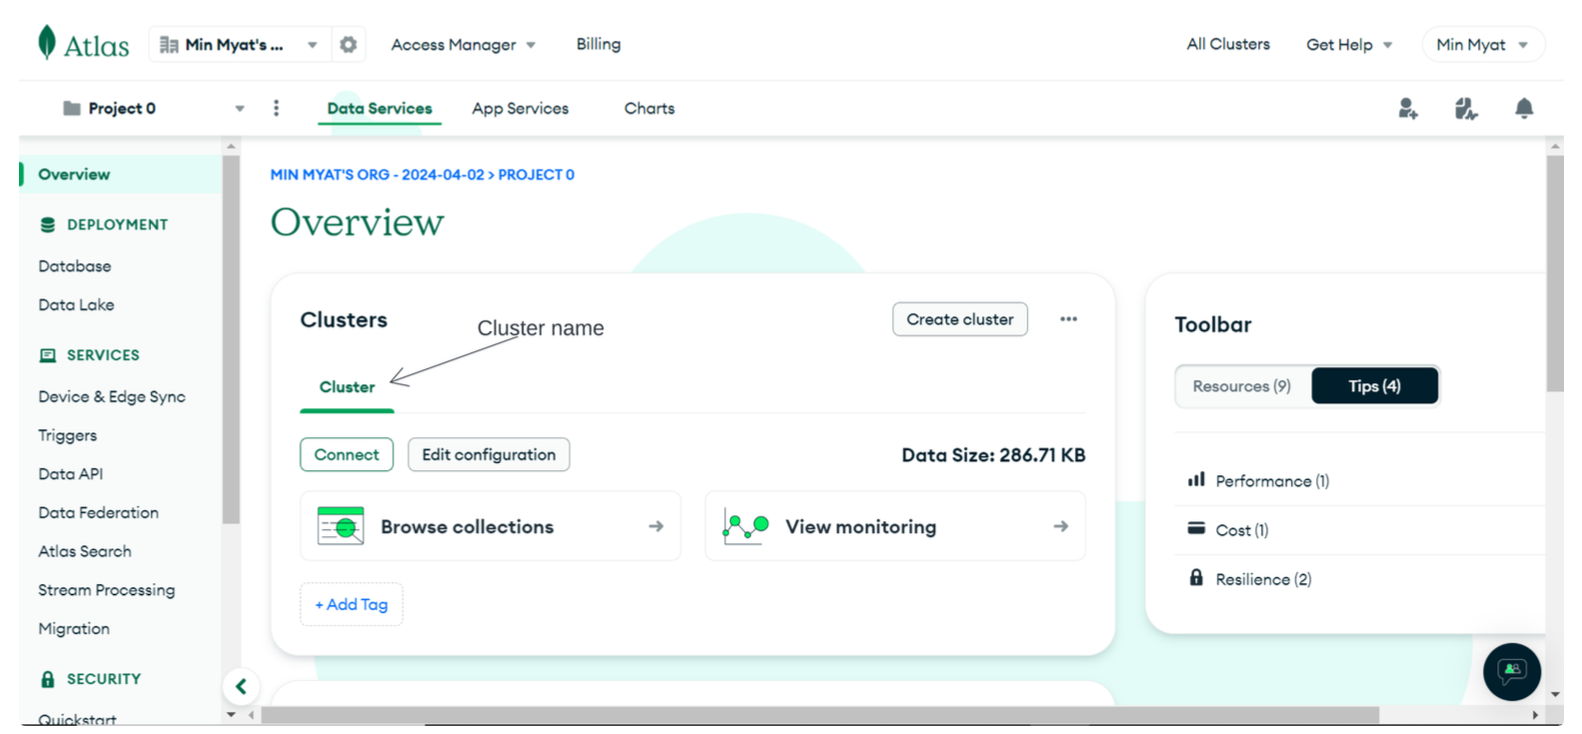
\includegraphics[width=1.0\textwidth,height=300px,frame]{cluster_name_example.png}
    \caption{How to Find Cluster Name}
    \label{fig:cluster_name}
    \end{figure}

    
    \item \textbf{Save the Connection String:}
    \begin{itemize}
        \item Store the modified connection string in the \texttt{.env} file as follows:
        
        \begin{verbatim}
        MONGO_DB_URL="your_connection_string_here"
        \end{verbatim}
    \end{itemize}
\end{enumerate}

Once these steps are completed, your database is ready for data input and output.






    \item \textbf{Stripe Integration:}
    \begin{itemize}
        \item Create an account at \texttt{https://stripe.com}.
        \item Obtain your API keys from the dashboard (see Figure~\ref{fig:stripe_api}).
        \item Configure the keys in your environment variables.
    \end{itemize}
    \begin{figure}[H]
	\centering	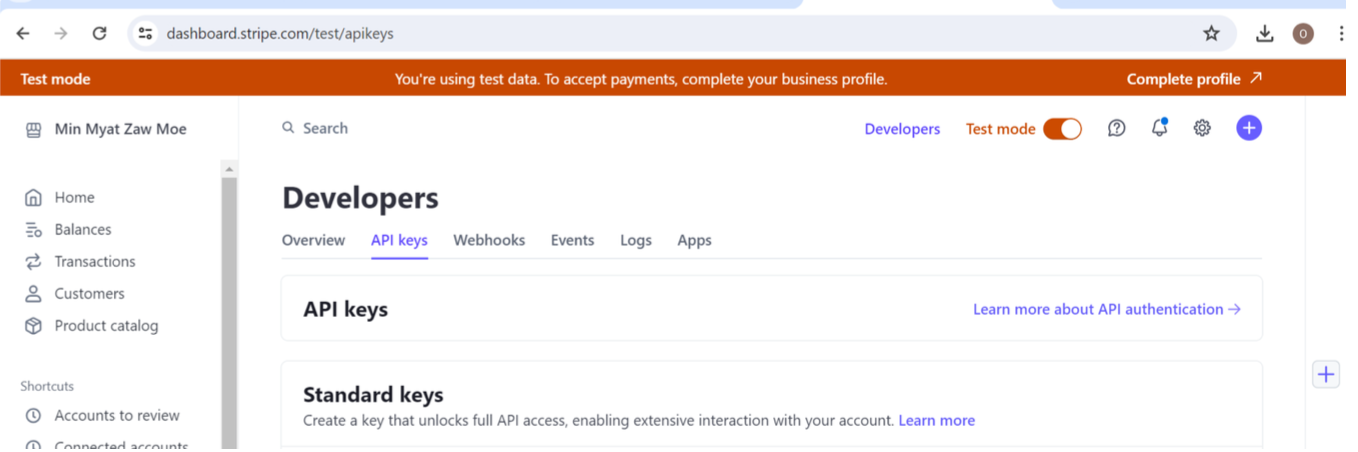
\includegraphics[width=1.0\textwidth,height=200px,frame]
    {stripeAPI.png}
    \caption{Stripe API Key}
    \label{fig:stripe_api}
    \end{figure}

    \item \textbf{Uploadthing Setup:}
    \begin{itemize}
        \item Sign up and create an account at \texttt{https://uploadthing.com}.
        \item Obtain your API key and configure it in the environment variables (see Figure~\ref{fig:ut_api}).
    \end{itemize}
    \begin{figure}[H]
	\centering	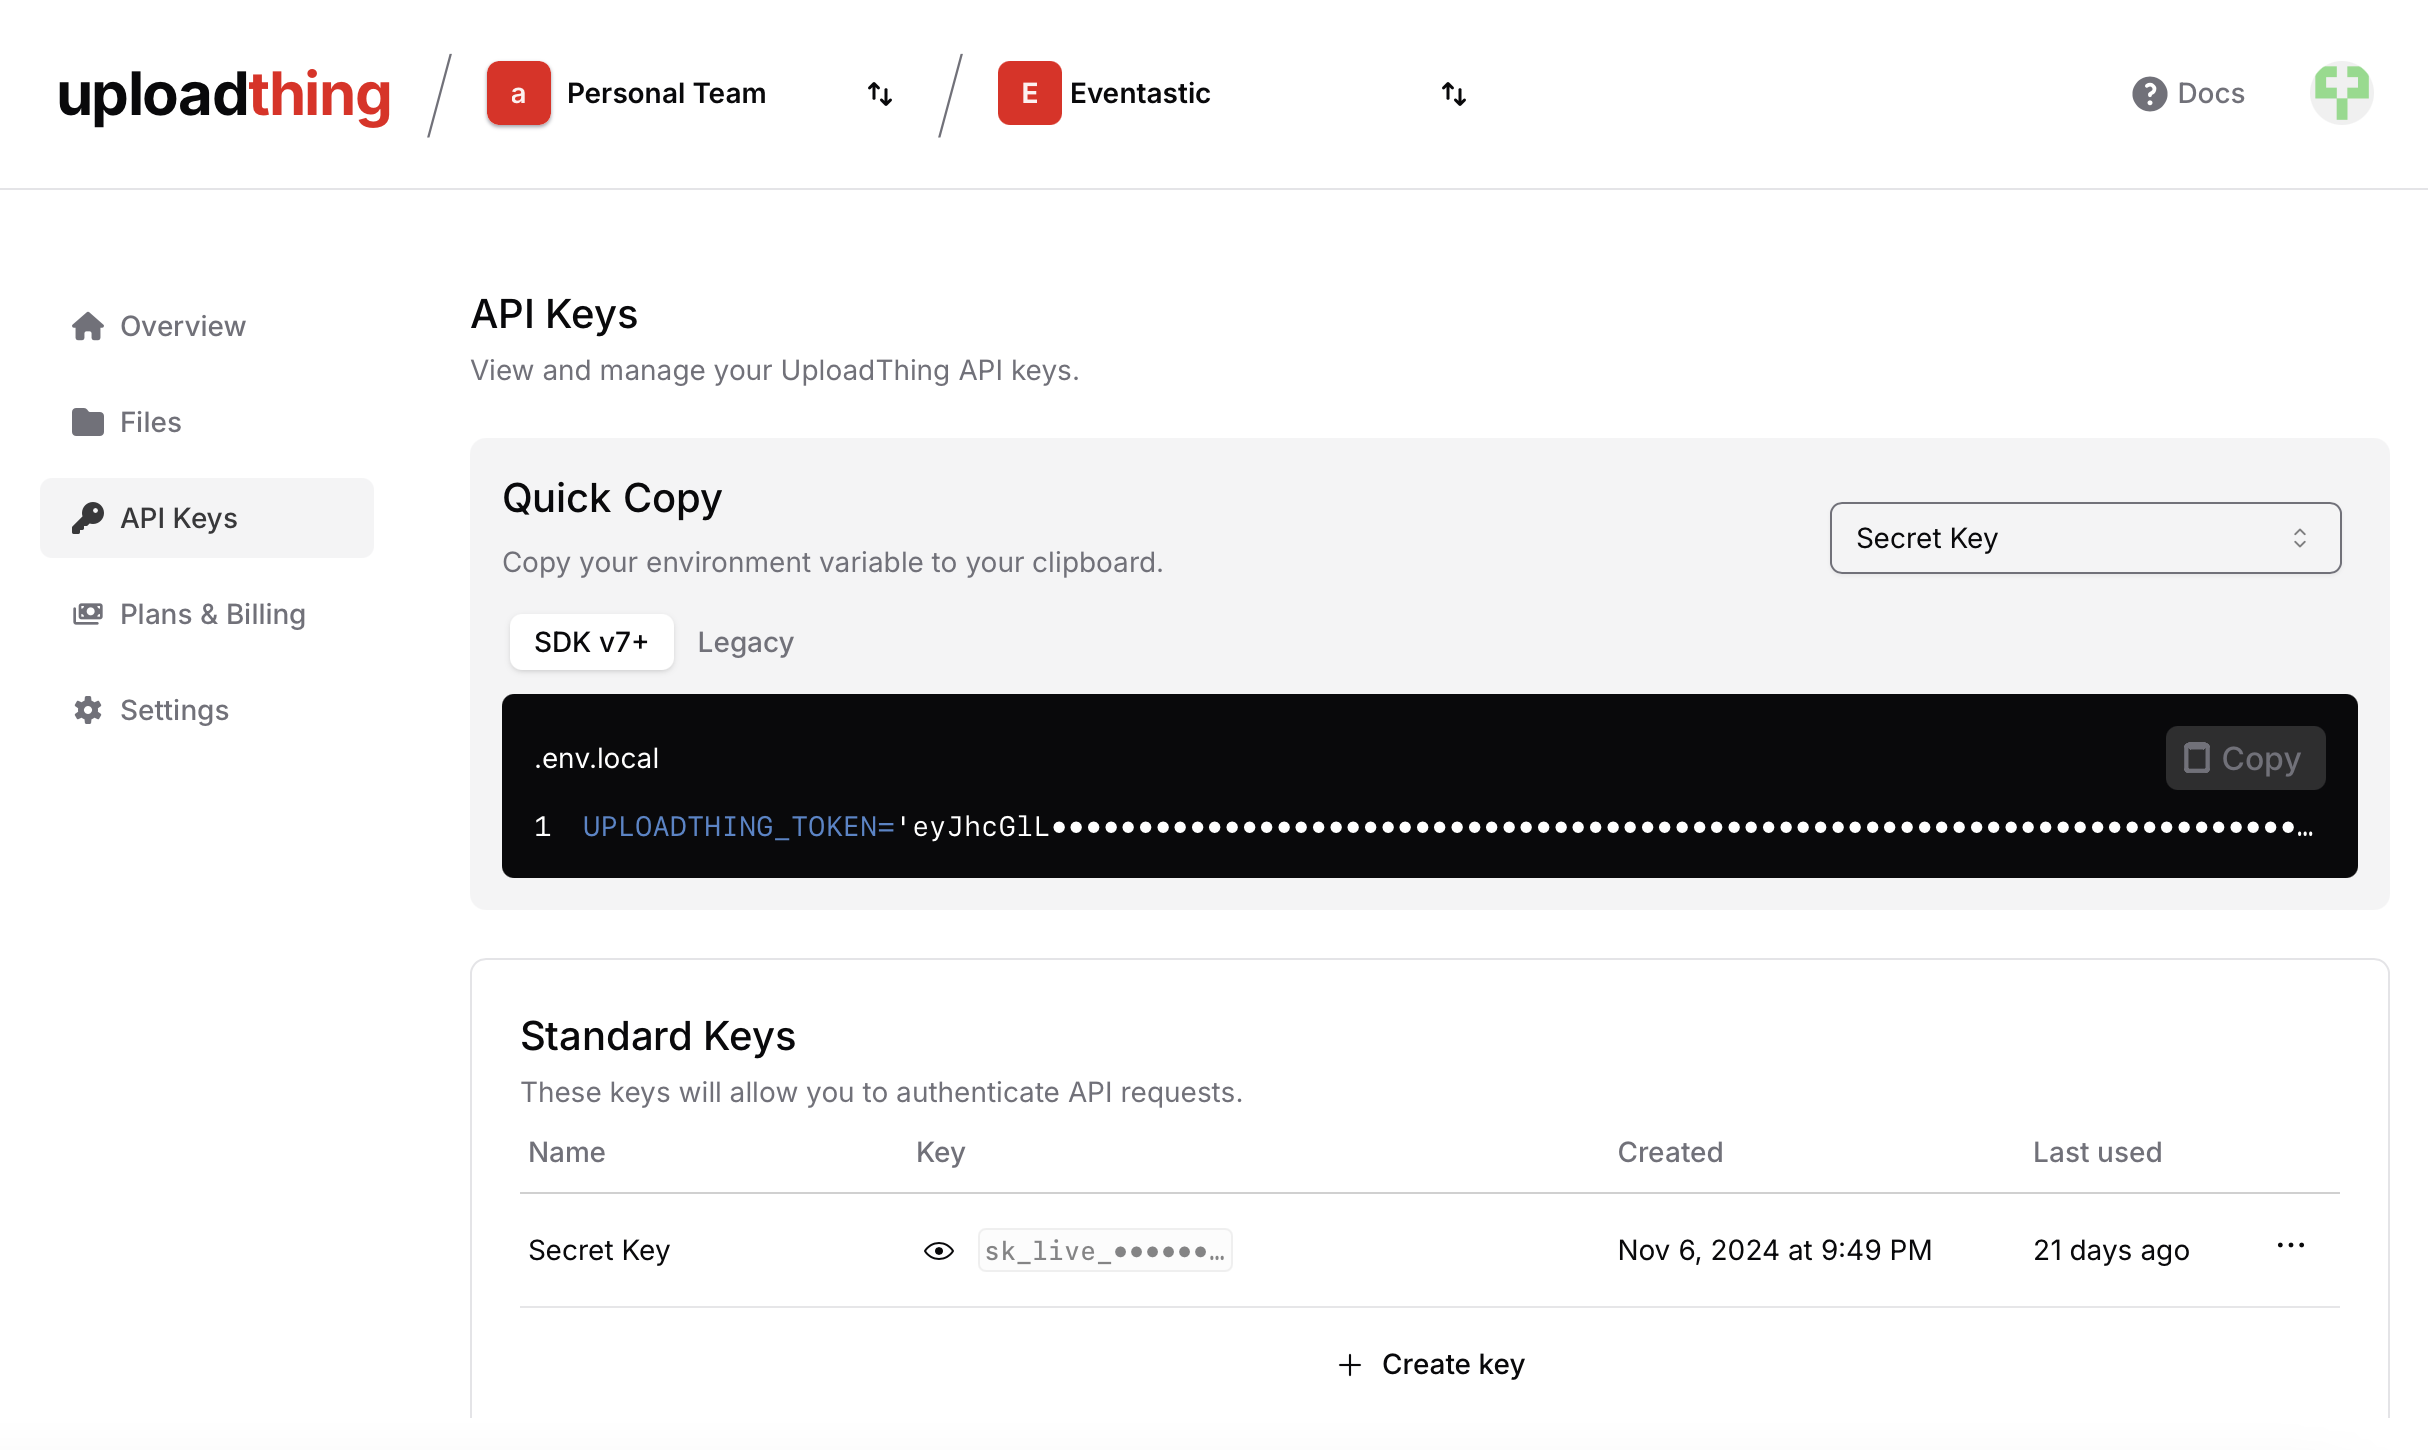
\includegraphics[width=1.0\textwidth,height=300px,frame]
    {utAPI.png}
    \caption{UploadThing API Key}
    \label{fig:ut_api}
    \end{figure}
    

    \item \textbf{Clerk Authentication:}
    \begin{itemize}
        \item Create an account at \texttt{https://clerk.dev}.
        \item Set up your application in the Clerk dashboard.
        \item Configure the required API keys in the environment file (see Figure~\ref{fig:clerk_api})).
    \end{itemize}
    \begin{figure}[H]
	\centering	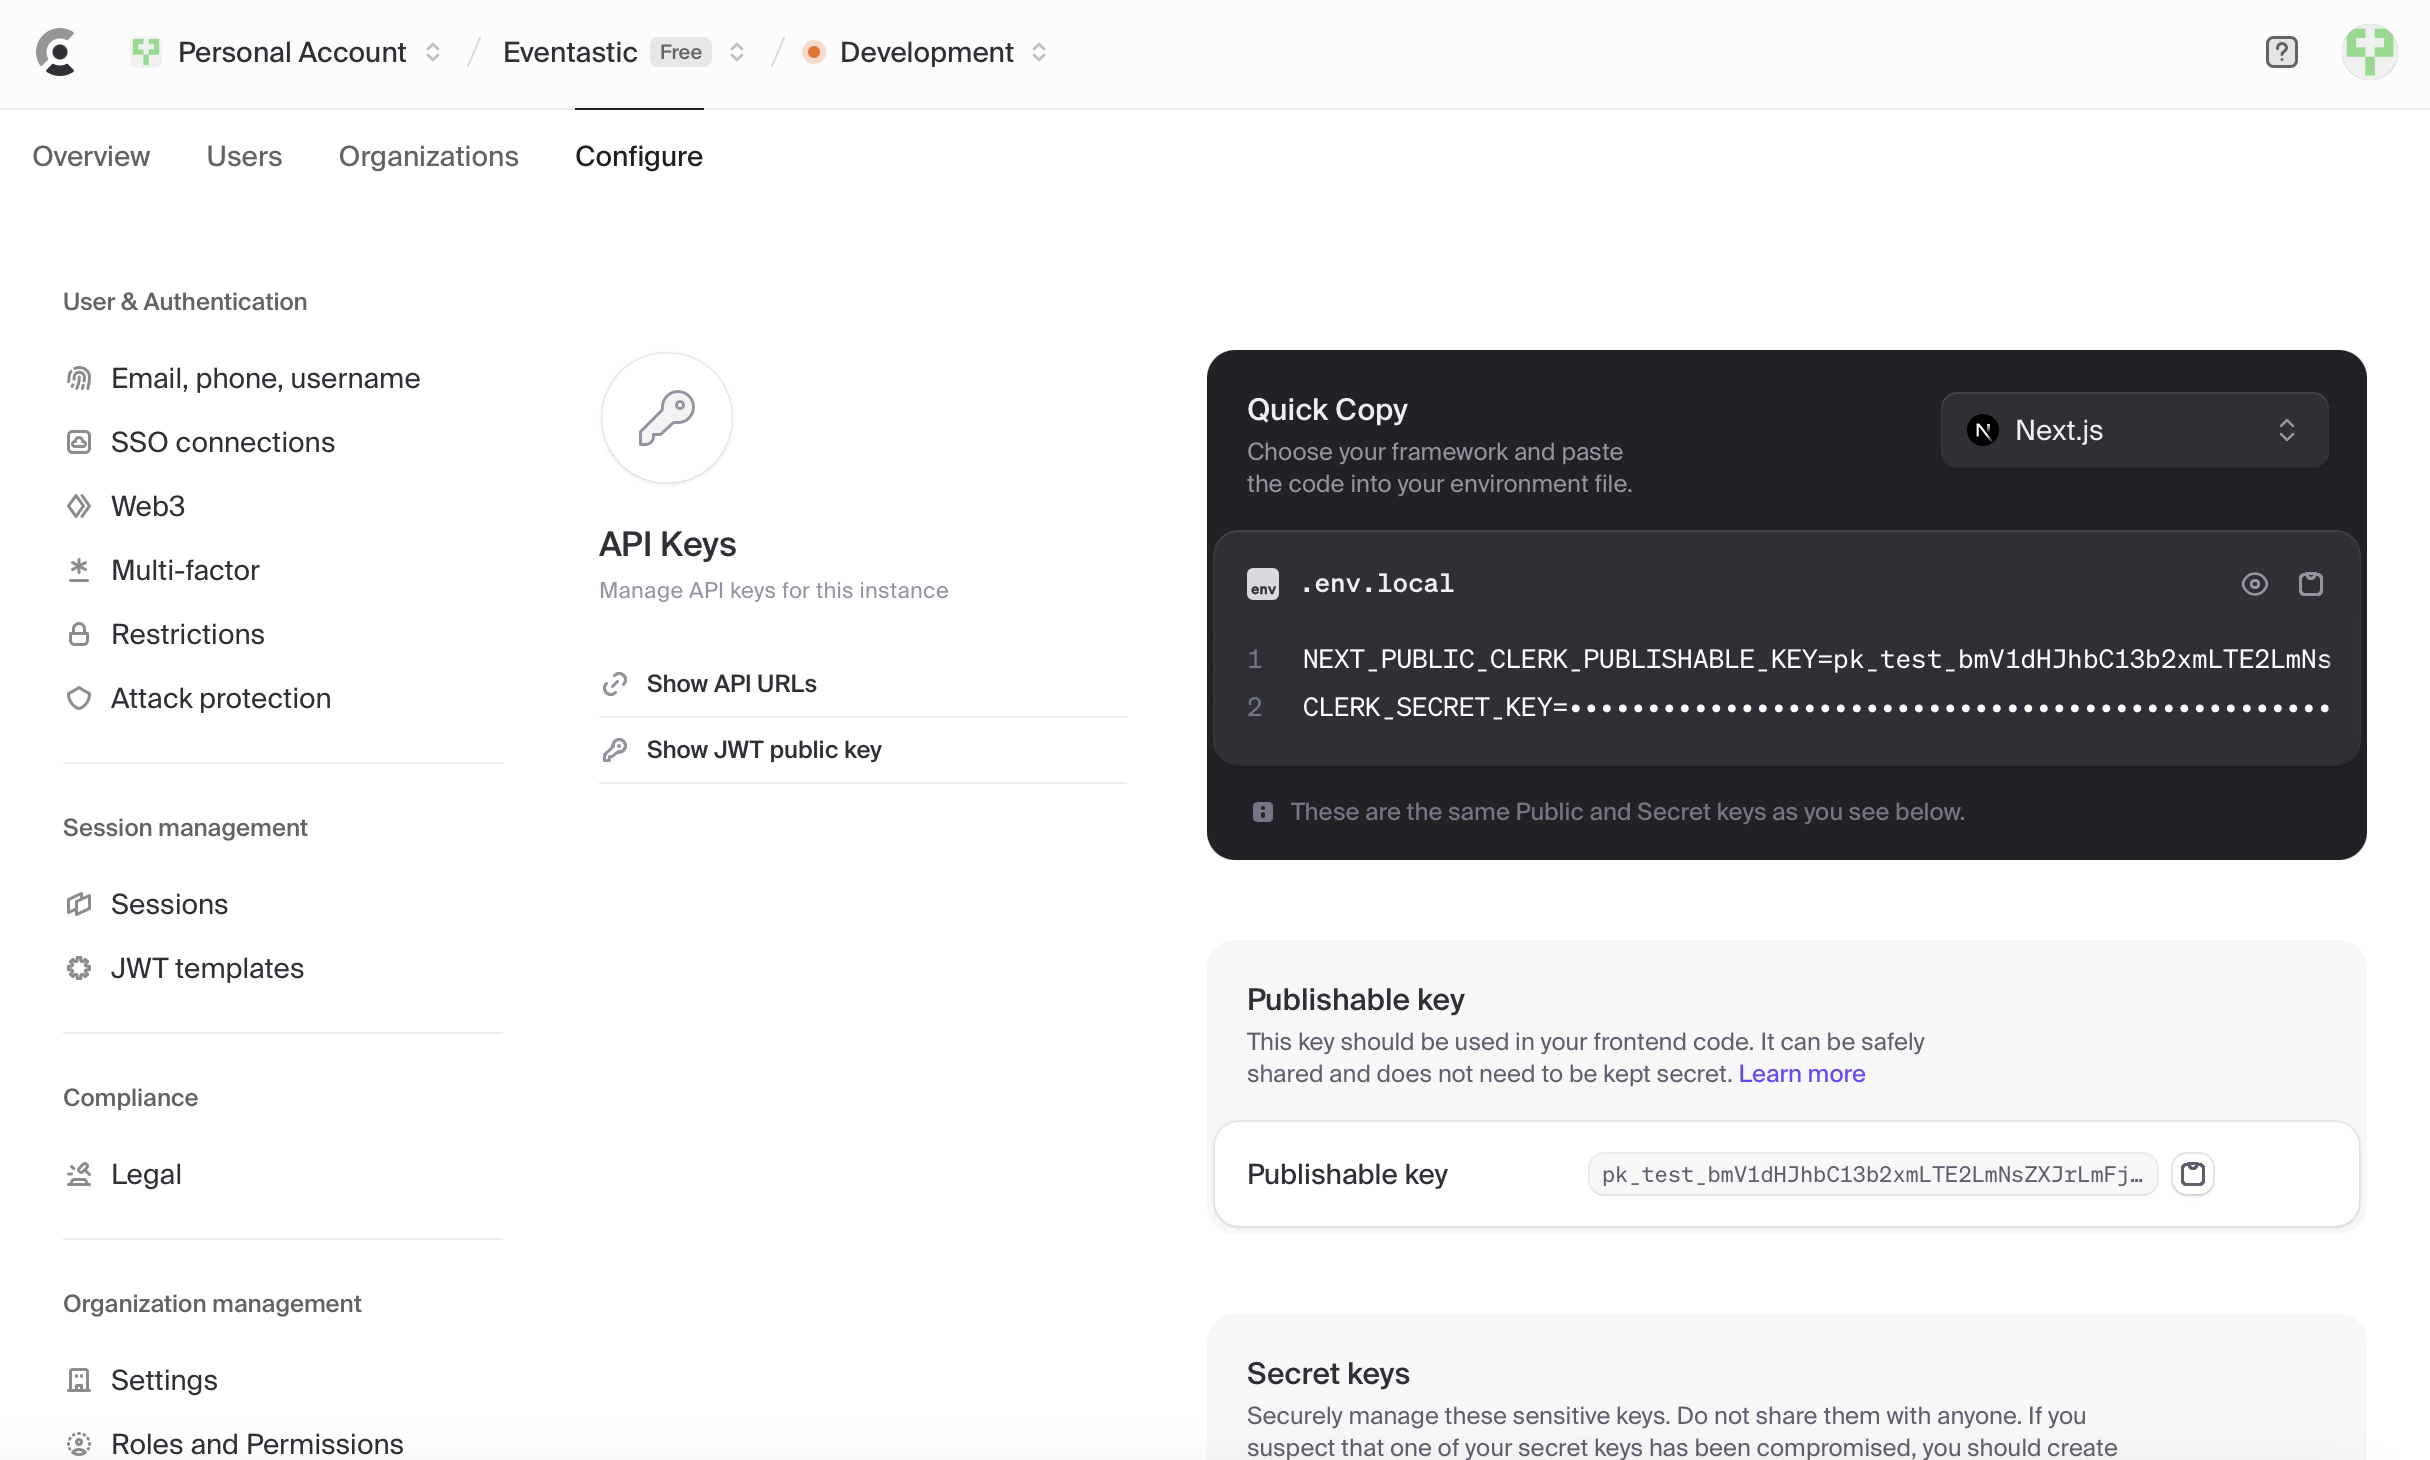
\includegraphics[width=1.0\textwidth,height=300px,frame]
    {clerkAPI.png}
    \caption{Clerk API Key}
    \label{fig:clerk_api}
    \end{figure}

    \item \textbf{Postman:}\cite{postman}
    \begin{itemize}
        \item Download Postman from \texttt{https://www.postman.com/downloads/}.
        \item Install and log in to start testing APIs.
    \end{itemize}

    \item \textbf{Git Setup:}
    \begin{itemize}
        \item Install Git from \texttt{https://git-scm.com/downloads}.
        \item Configure your username and email with the following commands:
        \begin{verbatim}
        git config --global user.name "Your Name"
        git config --global user.email "your.email@example.com"
        \end{verbatim}
    \end{itemize}
\end{enumerate}



If the reader has followed the steps outlined above, the development process can now begin. However, before diving into development, it is crucial to first understand the data models used in the application.

By familiarizing yourself with the data schema, you will gain a deeper insight into the workings of the API and the data presentation layers. This understanding will help clarify:
\begin{itemize}
    \item The structure and types of data being sent in API requests.
    \item The expected format and content of API responses.
\end{itemize}

This foundational knowledge will streamline your development efforts and ensure a more efficient interaction with the application’s backend services.






\section{Data Models}

This section provides a detailed overview of the data models used in the application.

\subsection{Category Model}

The \textbf{Category} model represents categories for events.

\begin{lstlisting}[style=typescript, caption={Category Model Interface}]
interface ICategory {
  _id: string;
  name: string;
}

Schema:
- _id: MongoDB ObjectId
- name: String (required)
\end{lstlisting}


\subsection{Event Model}

The \textbf{Event} model represents events in the system.

\begin{lstlisting}[style=typescript, caption={Event Model Interface}]
interface IEvent {
  _id: string;
  title: string;
  description?: string;
  location?: string;
  createdAt: Date;
  imageUrl: string;
  startDateTime: Date;
  endDateTime: Date;
  price: string;
  isFree: boolean;
  url?: string;
  category: { _id: string; name: string };
  organizer: { _id: string; firstName: string; lastName: string };
}

Schema:
- _id: MongoDB ObjectId
- title: String (required)
- description: String
- location: String
- createdAt: Date (default: Date.now)
- imageUrl: String (required)
- startDateTime: Date (required)
- endDateTime: Date (required)
- price: String (required)
- isFree: Boolean (required)
- url: String
- category: Reference to Category model
- organizer: Reference to User model
\end{lstlisting}


\subsection{Order Model}

The \textbf{Order} model represents event orders/tickets.

\begin{lstlisting}[style=typescript, caption={Order Model Interface}]
interface IOrder {
  _id: string;
  createdAt: Date;
  stripeId: string;
  totalAmount: string;
  event: { _id: string; title: string };
  buyer: { _id: string; firstName: string; lastName: string };
}

interface IOrderItem {
  _id: string;
  eventId: string;
  buyerId: string;
  totalAmount: string;
  createdAt: Date;
  stripeId: string;
}

Schema:
- _id: MongoDB ObjectId
- createdAt: Date (default: Date.now)
- stripeId: String (required)
- totalAmount: String (required)
- event: Reference to Event model
- buyer: Reference to User model
\end{lstlisting}

\subsection{User Model}

The \textbf{User} model represents user accounts in the system.

\begin{lstlisting}[style=typescript, caption={User Model Interface}]
interface IUser {
  _id: string;
  clerkId: string;
  email: string;
  username: string;
  firstName: string;
  lastName: string;
  photo: string;
}

Schema:
- _id: MongoDB ObjectId
- clerkId: String (unique, required)
- email: String (unique, required)
- username: String (unique, required)
- firstName: String (required)
- lastName: String (required)
- photo: String (required)
\end{lstlisting}

\subsection{Database Information}

The application uses \textbf{MongoDB} as its database, utilizing \textbf{Mongoose} as the ODM (Object Document Mapper). Each model is defined with TypeScript interfaces for type safety and Mongoose schemas for database structure. The models are interconnected through references, creating a relational structure within the MongoDB document database.


\section{Program}

The project leverages the \textbf{Next.js App Router} to maintain a clear structure and separation of concerns:
\begin{itemize}
    \item \texttt{app/}: Contains all page components and routing logic.
    \item \texttt{components/}: Houses reusable UI components.
    \item \texttt{lib/}: Includes server-side business logic and database interactions.
    \item \texttt{api/}: Defines API routes for external integrations.
\end{itemize}


While the codebase is not physically divided into separate repositories, it adheres to clear boundaries for maintainability:
\begin{itemize}
    \item \textbf{Front-end concerns}: Managed within the \texttt{app/} and \texttt{components/} directories.
    \item \textbf{Back-end logic}: Encapsulated within \texttt{lib/} and \texttt{api/}.
    \item \textbf{Database models}: Isolated in \texttt{lib/database/models/}.
    \item \textbf{Business logic actions}: Grouped within \texttt{lib/actions/}.
\end{itemize}



\subsection{Folder Structure}
The project follows a modern Next.js 14 application structure\cite{nextjs_project_structure} with a clear separation of concerns. Here's a detailed breakdown of the project organization:

\subsubsection{Root Directory Structure}

\begin{figure}[H]
	\centering	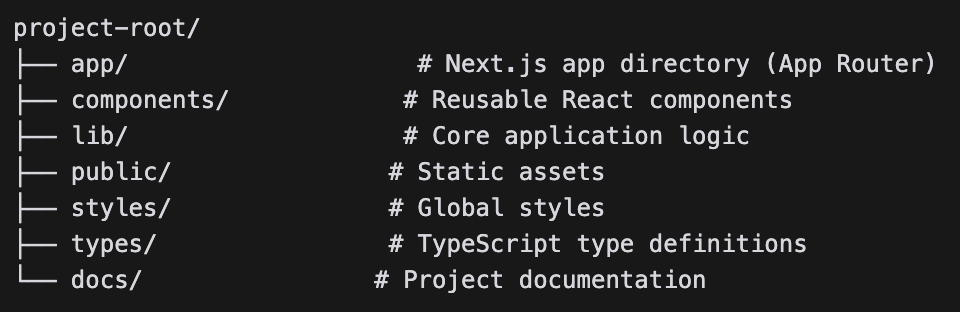
\includegraphics[width=1.0\textwidth,height=140px,frame]{rootdir.png}
    \caption{Root Directory Structure}
    \end{figure}


\subsubsection{Detailed Structure}

\begin{itemize}
    \item \textbf{App Directory (\texttt{/app})} \\
    The app directory utilizes Next.js 14 App Router architecture with the following structure: 
    \begin{figure}[H]
        \centering
        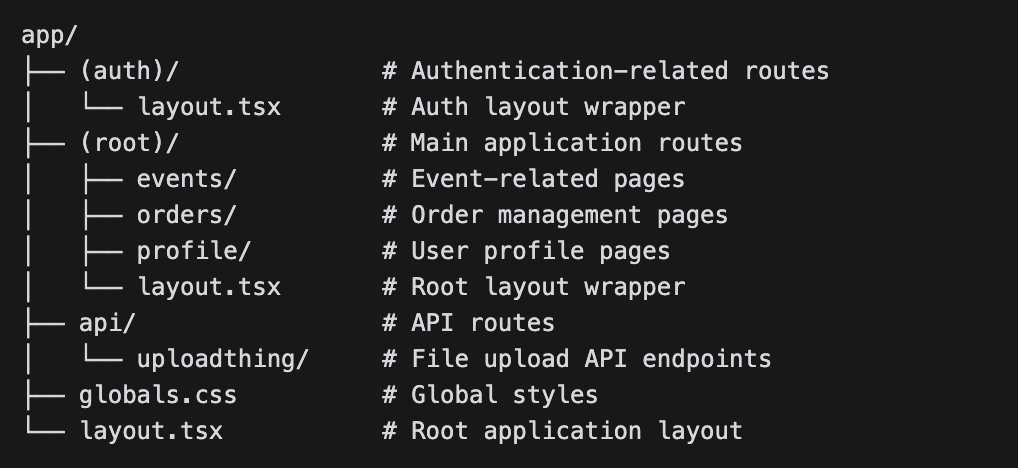
\includegraphics[width=1.0\textwidth,height=200px,frame]{appdir.png}
        \caption{App Directory Structure}
    \end{figure}

    \item \textbf{Components Directory (\texttt{/components})} \\
    The components directory contains reusable UI components:
    \begin{figure}[H]
        \centering
        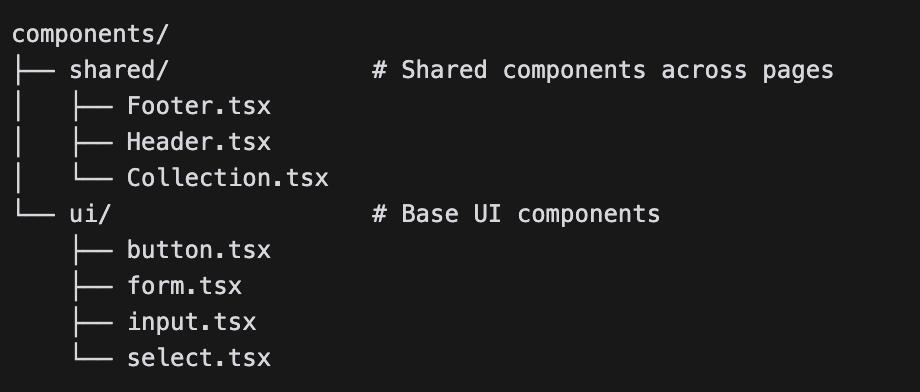
\includegraphics[width=1.0\textwidth,height=190px,frame]{componentsdir.png}
        \caption{Components Directory Structure}
    \end{figure}

    \item \textbf{Library Directory (\texttt{/lib})} \\
    The library directory includes utility functions and libraries:
    \begin{figure}[H]
        \centering
        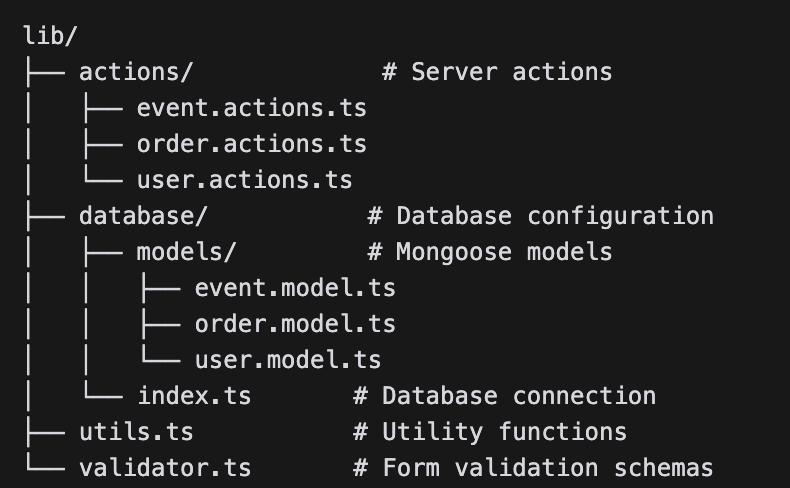
\includegraphics[width=1.0\textwidth,height=190px,frame]{libdir.png}
        \caption{Library Directory Structure}
    \end{figure}

    \item \textbf{Configuration Files} \\
    Key configuration files are located in the root directory:
    \begin{figure}[H]
        \centering
        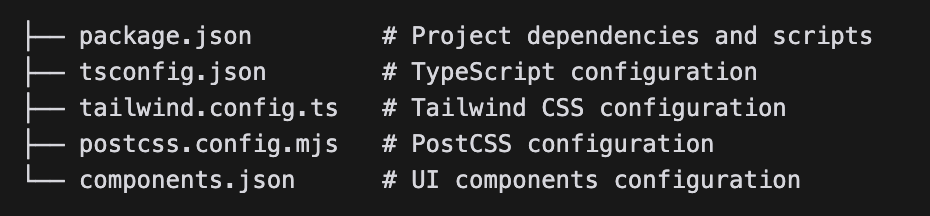
\includegraphics[width=1.0\textwidth,height=100px,frame]{configdir.png}
        \caption{Configuration Files}
    \end{figure}
\end{itemize}


\subsection{User Authentication System}
The application uses Clerk as its authentication provider, offering a robust and secure user management system. This integration provides a seamless authentication experience with features like email verification, social logins, and secure session management.

\subsubsection{Authentication Setup}
The project implements authentication using the following key components:
\begin{itemize}
    \item \textbf{Clerk Provider Configuration} 
\begin{lstlisting}[style=typescript, caption={Clerk Provider Configuration}]
    <ClerkProvider>
      <html lang="en">
        <body className={poppins.variable}>{children}</body>
      </html>
    </ClerkProvider>
  )
\end{lstlisting}

    \item \textbf{Protected Routes}  
    The middleware configuration controls access to different parts of the application:
\begin{lstlisting}[style=typescript, caption={middleware configuration routes}]
import { authMiddleware } from "@clerk/nextjs";
 
export default authMiddleware({
  publicRoutes: [
    '/',
    '/events/:id',
    '/api/webhook/clerk',
    '/api/webhook/stripe',
    '/api/uploadthing'
  ],
  ignoredRoutes: [
    '/api/webhook/clerk',
    '/api/webhook/stripe',
    '/api/uploadthing'
  ]
});
\end{lstlisting}


    
\end{itemize}


\subsubsection{User Registration Flow}
\begin{itemize}
    \item \textbf{Sign-Up Process}
    \begin{itemize}
    \item \textbf{Implemented through Clerk's built-in UI components:} Provides a pre-designed and customizable user interface for handling authentication workflows.
    \item \textbf{Automatic Email Verification:} Clerk handles email verification seamlessly without additional backend logic.
    \item \textbf{User Record Creation:} Upon successful registration, a webhook triggers the creation of a new user record in MongoDB.
    \item \textbf{Integration with Clerk:} Links the Clerk ID to the internal user database for consistent authentication and user profile management.
\end{itemize}

    \item \textbf{User Data Management}  
    When a new user registers, the system creates a user record in MongoDB with the following structure:
\begin{lstlisting}[style=typescript, caption={User Data Management}]
const UserSchema = new Schema({
  clerkId: { type: String, required: true, unique: true },
  email: { type: String, required: true, unique: true },
  username: { type: String, required: true, unique: true },
  firstName: { type: String, required: true },
  lastName: {type: String, required: true },
  photo: { type: String, required: true },
})
\end{lstlisting}



    \item \textbf{Webhook Integration}  
    The system handles user lifecycle events through webhooks:
\begin{lstlisting}[style=typescript, caption={Webhook Integration}]
  if(eventType === 'user.created') {
    const { id, email_addresses, image_url, first_name, last_name, username } = evt.data;

    const user = {
      clerkId: id,
      email: email_addresses[0].email_address,
      username: username!,
      firstName: first_name,
      lastName: last_name,
      photo: image_url,
    }

    const newUser = await createUser(user);

    if(newUser) {
      await clerkClient.users.updateUserMetadata(id, {
        publicMetadata: {
          userId: newUser._id
        }
      })
    }

    return NextResponse.json({ message: 'OK', user: newUser })
  }
\end{lstlisting}    
\end{itemize}

\subsubsection{Login System}
\paragraph{1. Authentication Components}
\begin{itemize}
    \item Sign-in page using Clerk's pre-built components
    \item Secure session management
    \item Automatic token handling
\end{itemize}

\paragraph{2. Protected Routes}
\begin{itemize}
    \item Access control based on authentication status
    \item Public routes accessible without authentication
    \item Protected routes requiring user login
\end{itemize}




\section{Testing}

To ensure comprehensive coverage of our platform's features, the test cases are divided into four distinct categories: users, events, orders, and payments.

\textbf{Remark:} Testing is conducted using actual HTTP requests to our application via the \texttt{supertest}\cite{supertest} package. Consequently, data changes are reflected in the database. To prevent data pollution, it is advisable to use mock objects with distinguishable properties. Therefore, mock test data is utilized for executing test cases.

There is a specific order for running the test files because the outcomes of some cases serve as prerequisites for subsequent cases. Since test cases run asynchronously, we cannot guarantee execution in the order they are written. Therefore, the test files should be executed sequentially. The recommended order is:
\begin{enumerate}
    \item \texttt{user.test.ts}
    \item \texttt{event.test.ts}
    \item \texttt{order.test.ts}
    \item \texttt{payment.test.ts}
\end{enumerate}

Another precaution is that some test cases will only work once. This occurs in registration test cases, where a negative test expecting an unregistered email may fail if the email was registered in a previous run.

To reset the test files to a 100\% correct state, we need to delete the mock data manually or programmatically. This can be achieved by:
\begin{itemize}
    \item Manually removing the mock documents in the MongoDB dashboard.
    \item Programmatically deleting users, events, and orders with the properties of the provided mock data using the \texttt{deleteMany}\cite{mongoose_deletemany} function (as seen below) from Mongoose, with appropriate predicates.
\end{itemize}

\vspace{1cm}
\begin{lstlisting}[style=typescript, caption={Example Code for Deleting Mock Data}]
import mongoose from 'mongoose';
import User from './models/user.model';
import Event from './models/event.model';
import Order from './models/order.model';

async function deleteMockData() {
  await mongoose.connect(process.env.MONGODB_URI);

  // Delete mock users
  await User.deleteMany({ email: /mockuser@/ });

  // Delete mock events
  await Event.deleteMany({ title: /Mock Event/ });


  // Delete mock orders
  await Order.deleteMany({ stripeId: /mockStripeId/ });

  console.log('Mock data deleted successfully');
  await mongoose.disconnect();
}

deleteMockData().catch(console.error);
\end{lstlisting}   

\subsection{User Test Cases}
The first test suite is about customer. The scenarios include :
\begin{itemize}
    \item Registration
    \item Logging In
    \item Event Registration
\end{itemize}

\vspace{1cm}

\subsubsection{Registration}
\begin{itemize}
    \item \textbf{Objective:} To test user registration.
    \item \textbf{Precondition:} The database should not contain mock user data.
    \item \textbf{Expected Result:} Mock user is now recorded in the database.
    \item \textbf{Test Steps:}
    \begin{itemize}
        \item Test registration with a new email (expected to succeed).
        \item Test registration with an already-registered email (expected to return an error).
    \end{itemize}
\end{itemize}

\begin{lstlisting}[style=typescript, caption={Mock Test Data - User}]
const mockUser = {
  _id: "mockUserId",
  clerkId: "mockClerkId",
  email: "mockUser@gmail.com",
  username: "mockUser",
  firstName: "Mock",
  lastName: "User",
  photo: "https://example.com/photo.jpg"
}
\end{lstlisting}  

\subsubsection{Logging In}
\begin{itemize}
    \item \textbf{Objective:} To test the login feature.
    \item \textbf{Precondition:} The database should have mock user data recorded.
    \item \textbf{Expected Result:} 
    \begin{itemize}
        \item Invalid credentials error for incorrect email and password.
        \item A user data object for login attempts with correct mock user data.
    \end{itemize}
    \item \textbf{Test Steps:}
    \begin{itemize}
        \item Test both positive and negative cases.
        \item Check the response code and returned information for all scenarios.
    \end{itemize}
\end{itemize}

\subsubsection{Event Registration}
\begin{itemize}
    \item \textbf{Objective:} User can register for events.
    \item \textbf{Precondition:} The database should have mock user and event data recorded.
    \item \textbf{Expected Result:} 
    \begin{itemize}
        \item The event registration is saved under the user in the database.
        \item Verify the registration by retrieving the user's registered events.
    \end{itemize}
    \item \textbf{Test Steps:}
    \begin{itemize}
        \item Test with valid event IDs (expected to succeed).
        \item Test with invalid event IDs (expected to fail).
    \end{itemize}
\end{itemize}


\subsection{Event Organizer Test Cases} The second test suite is about event organizers. The scenarios include: \begin{itemize} \item Creating an Event \item Managing Event Registrations \end{itemize}

\vspace{1cm}

\subsubsection{Creating an Event}
\begin{itemize}
    \item \textbf{Objective:} Organizers can create events.
    \item \textbf{Precondition:} The database should have mock organizer data recorded.
    \item \textbf{Expected Result:}
    \begin{itemize}
        \item The event is successfully created and recorded in the database for valid data.
        \item An error is returned for invalid event data.
    \end{itemize}
    \item \textbf{Test Steps:}
    \begin{itemize}
        \item Test creating an event with valid data (expected to succeed).
        \item Test creating an event with invalid data (expected to return an error).
    \end{itemize}
\end{itemize}

\begin{lstlisting}[style=typescript, caption={Mock Test Data - Event}]
const mockEvent = {
  _id: "mockEventId",
  title: "Mock Event",
  description: "This is a mock event for testing.",
  location: "Budapest",
  createdAt: 2024-11-06T20:11:01.888+00:00,
  imageUrl: "https://example.com/event.jpg",
  startDateTime:2025-02-21T14:20:00.000+00:00,
  endDateTime: 2025-02-21T16:20:00.000+00:00,
  price: "20",
  isFree: false,
  url: "https://example.com",
  category: { _id: "mockCategoryId", name: "AI" },
  organizer: { _id: "mockOrganizerId", firstName: "Mock", lastName: "Organizer" }
}
\end{lstlisting}  

\subsubsection{Managing Event Registrations}
\begin{itemize}
    \item \textbf{Objective:} Organizers can view and manage event registrations.
    \item \textbf{Precondition:} The database should have mock event and registration data recorded.
    \item \textbf{Expected Result:}
    \begin{itemize}
        \item The organizer can successfully retrieve event registrations for valid event IDs.
        \item An error is returned for invalid event IDs.
    \end{itemize}
    \item \textbf{Test Steps:}
    \begin{itemize}
        \item Test retrieving registrations with valid event IDs (expected to succeed).
        \item Test retrieving registrations with invalid event IDs (expected to return an error).
    \end{itemize}
\end{itemize}


\subsection{Event Test Cases}
The third test suite is about events. The scenarios include:
\begin{itemize}
    \item Listing Events
    \item Getting a Specific Event
\end{itemize}

\vspace{1cm}

\subsubsection{Listing Events}
\begin{itemize}
    \item \textbf{Objective:} Event collections can be fetched successfully.
    \item \textbf{Precondition:} The database should have mock events recorded.
    \item \textbf{Expected Result:}
    \begin{itemize}
        \item A list of events is returned that matches the query criteria, such as title, category, and date range.
    \end{itemize}
    \item \textbf{Test Steps:}
    \begin{itemize}
        \item Test fetching events with different query parameters (expected to succeed).
        \item Validate that returned events match the specified queries.
    \end{itemize}
\end{itemize}


\subsubsection{Getting a Specific Event}
\begin{itemize}
    \item \textbf{Objective:} Single event fetch returns event information.
    \item \textbf{Precondition:} The database should have mock event data recorded.
    \item \textbf{Expected Result:}
    \begin{itemize}
        \item The event data is returned for valid event IDs.
        \item An error is returned for invalid event IDs.
    \end{itemize}
    \item \textbf{Test Steps:}
    \begin{itemize}
        \item Test fetching event data with a valid event ID (expected to succeed).
        \item Test fetching event data with an invalid event ID (expected to return an error).
    \end{itemize}
\end{itemize}



\subsection{Payment Test Cases}
The fourth test suite is about payments. The scenario includes:
\begin{itemize}
    \item Processing Payments
\end{itemize}

\vspace{1cm}

\subsubsection{Processing Payments}
\begin{itemize}
    \item \textbf{Objective:} To test the payment processing.
    \item \textbf{Precondition:} None.
    \item \textbf{Expected Result:}
    \begin{itemize}
        \item A payment session ID is generated.
        \item A payment session URL is returned for the created order.
    \end{itemize}
    \item \textbf{Test Steps:}
    \begin{itemize}
        \item Test creating an order with mock payment data.
        \item Validate that the response contains a valid payment session ID and URL.
    \end{itemize}
\end{itemize}

\begin{lstlisting}[style=typescript, caption={Mock Test Data - Order}]
const mockOrder = {
  _id: "mockOrderId",
  createdAt: 2025-02-21T14:20:00.000+00:00,
  stripeId: "mockStripeId",
  totalAmount: "50.00",
  event: {
    _id: "mockEventId",
    title: "Mock Event"
  },
  buyer: {
    _id: "mockBuyerId",
    firstName: "Mock",
    lastName: "Buyer"
  }
}

const mockOrderItem = {
  _id: "mockOrderItemId",
  eventId: "mockEventId",
  buyerId: "mockBuyerId",
  totalAmount: "50.00",
  createdAt: 2025-02-21T14:20:00.000+00:00,
  stripeId: "mockStripeId"
}
\end{lstlisting}  


We have now completed the developer documentation for the event management web application. By this point, the reader should have a clear understanding of the internal workings of the platform and be prepared for further development. In case of any issues or questions, the author can be contacted at blvhi9@inf.elte.hu. The next section will summarize the project and explore potential future directions.

